The company ONAR MMSoft is a company that located at Jouy-en-Josas, France.
It's part of a bigger company, ONAR MMCall, which specializes in the distribution
of pagers, in as a complement to this offering software that can blend with the pagers.

As of today, the company has interest in several fields of activities:

\begin{center}
    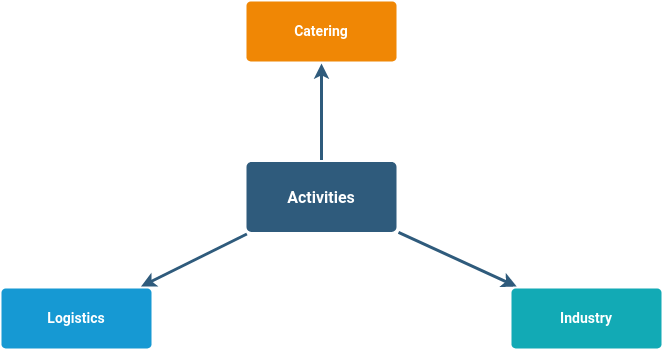
\includegraphics[width=0.8\textwidth]{images/core_activities.png}
\end{center}

Mainly handling the problems of management of part of the workflows in all these fields. 
And lately turning all their focus into logistics.

Some of the solutions that the company has developed and is maintaining are:

Ultim R which is composed of an App to order lunch, an IT tool to manage kitchen operations
from dishes preparation to order management and a module for plates delivery which was for
the client RATP.

Easy Truck In a solution for the management of trucks, which is a winner of an ID Logistics
interval innovation contest, it provides easy access to the logistics platform, support
operational teams, eases check-in and access controls and lastly has full support to
visual management.

Finally, there was solution for Autoneum which was a solution focused on reducing the time
spent with production workstations on factories.

\begin{center}
    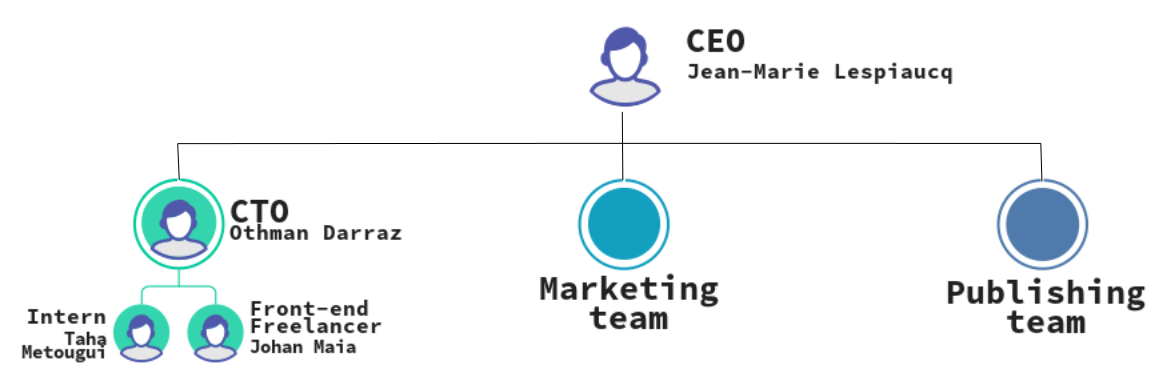
\includegraphics[width=0.85\textwidth]{images/Hierarchy}
\end{center}

The team, I've integrated, is composed of a team of 2 people, the CTO Othman Darraz who's
in charge of managing the project and a freelancer Johan who's in charge of everything that's
front related, and me joining them as the third member of the team taking care of backend
mainly refactoring, optimization and security.


